\documentclass[11pt,letterpaper]{article}
\usepackage[margin=1in]{geometry}
\usepackage{graphicx}
\usepackage{hyperref}
\usepackage{listings}
\usepackage{amsmath}
\pagestyle{headings}
\usepackage{epstopdf}

\begin{document}

\title{PHY 410 \\ Homework Assignment 10}
\author{Han Wen \\ \tiny Person No. 50096432}
\date{\today}

\maketitle

\begin{abstract}
The goal of this assignment is to get more familiar with random process and method, as well as its application on random walk and statistical mechanics.


\end{abstract}

\tableofcontents

\newpage
\section{Problem 1}

\subsection{Description}

Modify rwalk.cpp or rwalk.py to simulate a random walk on a 2-dimensional square lattice and a 3-dimensional cubic lattice. Measure the diffusion constant D in 2 and 3 dimensions and compare with the 1-dimensional walk and theoretical expectations.

\subsection{Numerical result and analysis}


Theoretically, for example in one dimension, assume for each step the displacement will be $\pm\delta$, thus the position after N steps can be expressed as:
$$
x^2(N)=[x(N-1)\pm\delta]^2 = x^2(N+1) \pm 2\delta{x}(N-1)+{\delta}^2
$$
Thus the average will be:
$$
\big \langle {x^2(N)} \big \rangle= \big \langle {x^2(N-1)} \big \rangle \pm 2{\delta}x(N-1) + {\delta}^2
$$

the middle term is zero, therefore we have:
$$
\big \langle {x^2(N)} \big \rangle= \big \langle {x^2(N-1)} \big \rangle + {\delta}^2
$$

consequently:
$$
\big \langle {x^2(N)} \big \rangle= N{\delta}^2
$$
In 2 and 3 dimensions it is nothing but the summation in each individual direction. 
In my case, for each step the displacement in x, y, z direction is 1, therefore the diffusion constants for 1, 2, 3 dimensions are 0.5, 1, 1.5.


Modify the code to simulate for 2 and 3 dimensions, for 2 dimensions, since the random number generator is not a perfect one and limited by the number of steps, when using 1000 ensembles and 1000 steps the result is $1.017\pm0.001$ Fig. ~\ref{figure1} , while using 10000, 10000 setting, the result is $0.9990\pm0.0001$very close to theoretical value. Fig ~\ref{figure2}


\begin{figure}
\begin{center}
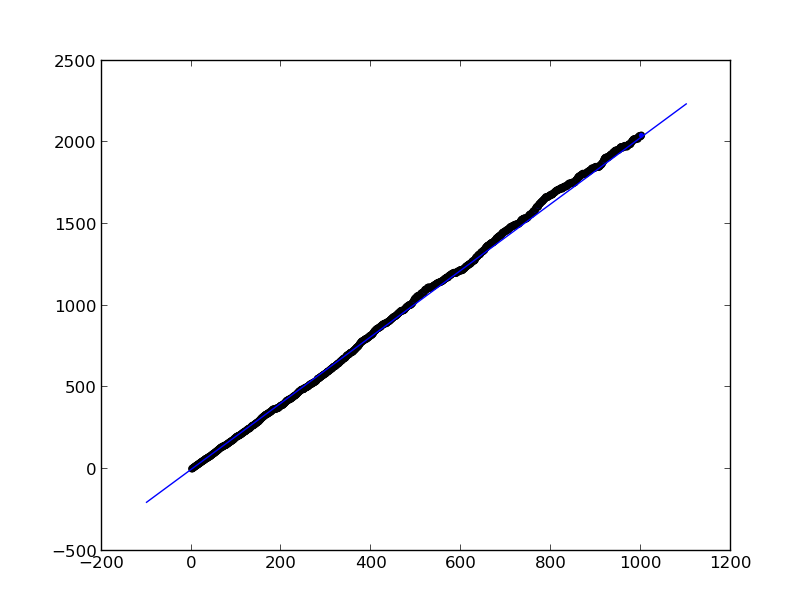
\includegraphics[width=0.8\linewidth,angle=0]{p11.png}
\caption{2d average of $displacement^2$ vs. steps, 1000 walkers}
\label{figure1}
\end{center}
\end{figure}


\begin{figure}
\begin{center}
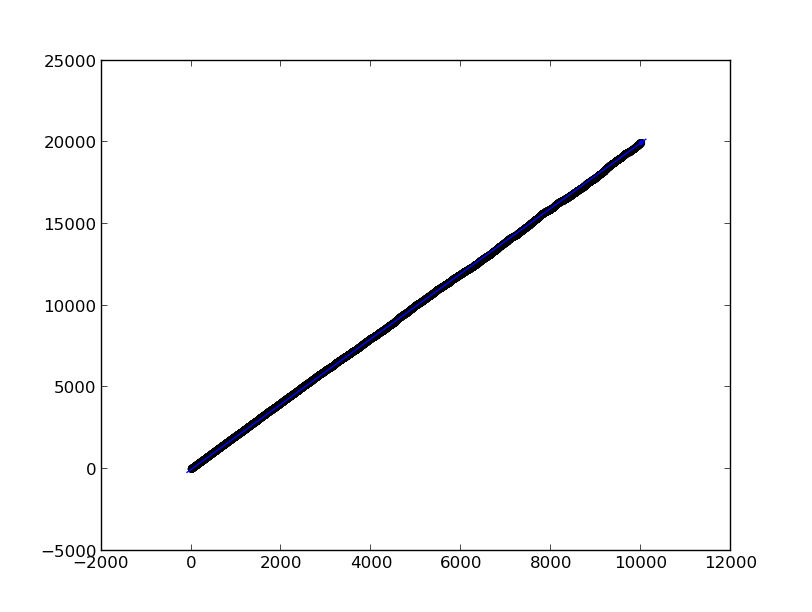
\includegraphics[width=0.8\linewidth,angle=0]{p12.png}
\caption{2d average of $displacement^2$ vs. steps, 10000 walkers}
\label{figure2}
\end{center}
\end{figure}

For 3 dimensions: for 1000 walkers 1000 steps, the result is $1.499 \pm 0.001$ Fig. ~\ref{figure3}

Since it is a random process, each time the result will be different and roughly fluctuating around the theoretical value, I was quite lucky in this trial, thus I stopped here.
\begin{figure}
\begin{center}
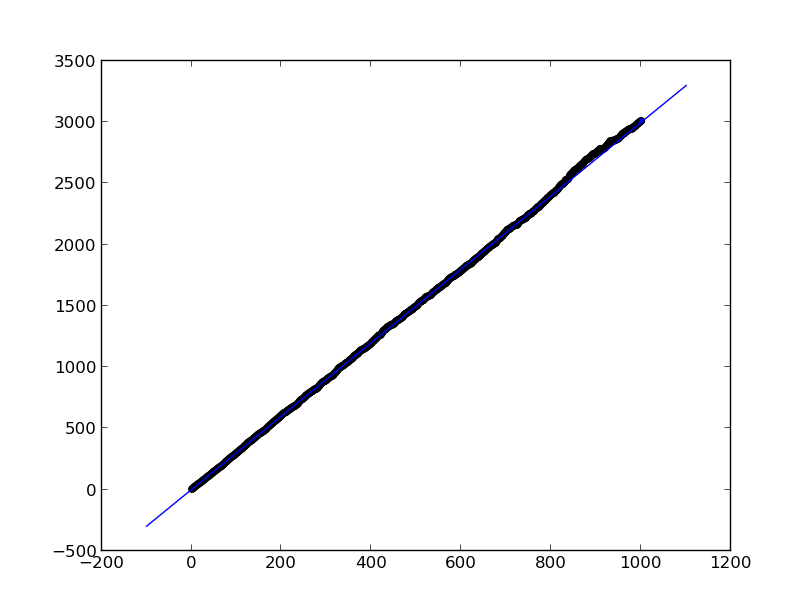
\includegraphics[width=0.8\linewidth,angle=0]{p13.png}
\caption{3d average of $displacement^2$ vs. steps, 1000 walkers}
\label{figure3}
\end{center}
\end{figure}






\newpage

\section{Problem 2}

\subsection{Description}
Measure and plot the average magnetization $\big \langle |M| \big \rangle$  and Heat Capacity C  of the Ising model as a function of temperature  T for three different lattice sizes. Use the data to identify the transition temperature $T_C$ .

\subsection{Result}

I used the lattice of size 10x10, 50x50, 100x100, using 500 MC steps.(This is a fair number for 10x10 yet not sufficient for larger grids, however, limited by the performance even using c++, I chose this number, we can see below for large grids the result is not so obvious)

For 10x10: Fig. ~\ref{figure4}
For 50x50: Fig. ~\ref{figure5}
For 100x100: Fig. ~\ref{figure5}

\begin{figure}
\begin{center}
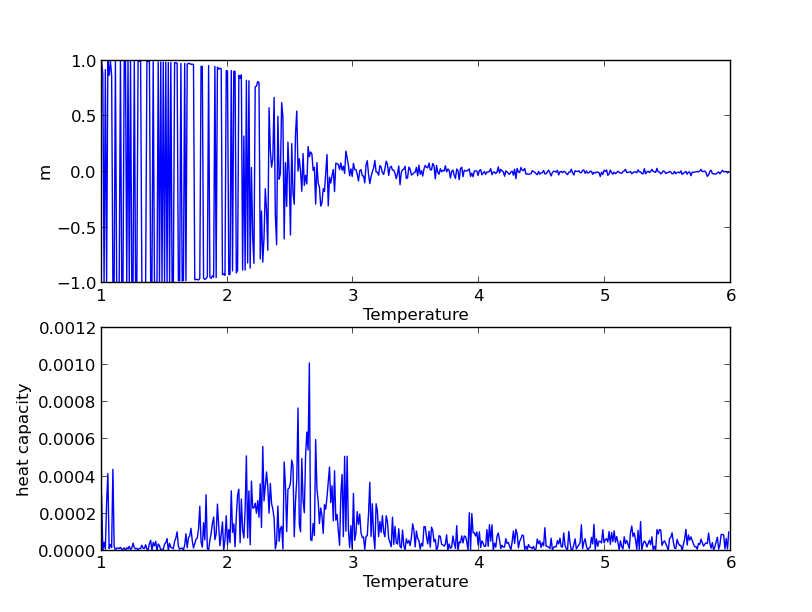
\includegraphics[width=0.8\linewidth,angle=0]{cp210.png}
\caption{10x10 lattice m and c vs. T}
\label{figure4}
\end{center}
\end{figure}


\begin{figure}
\begin{center}
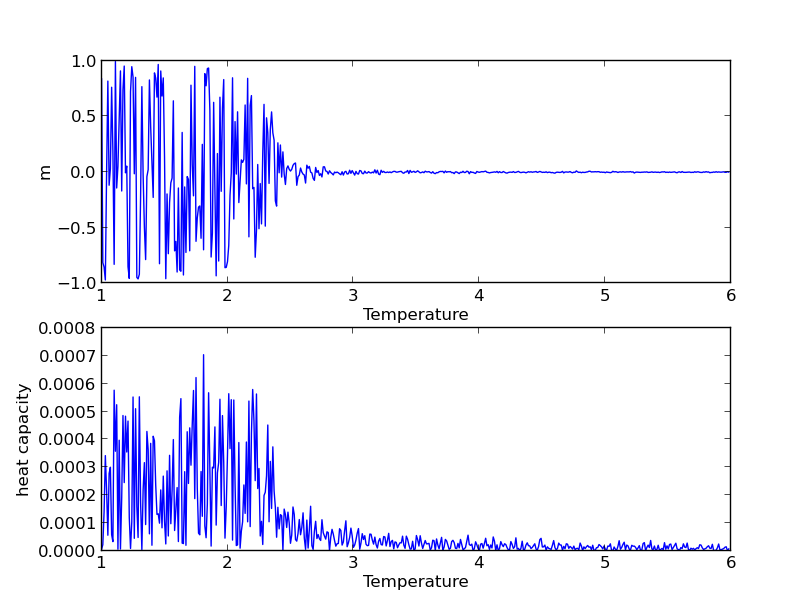
\includegraphics[width=0.8\linewidth,angle=0]{cp250.png}
\caption{50x50 lattice m and c vs. T}
\label{figure5}
\end{center}
\end{figure}


\begin{figure}
\begin{center}
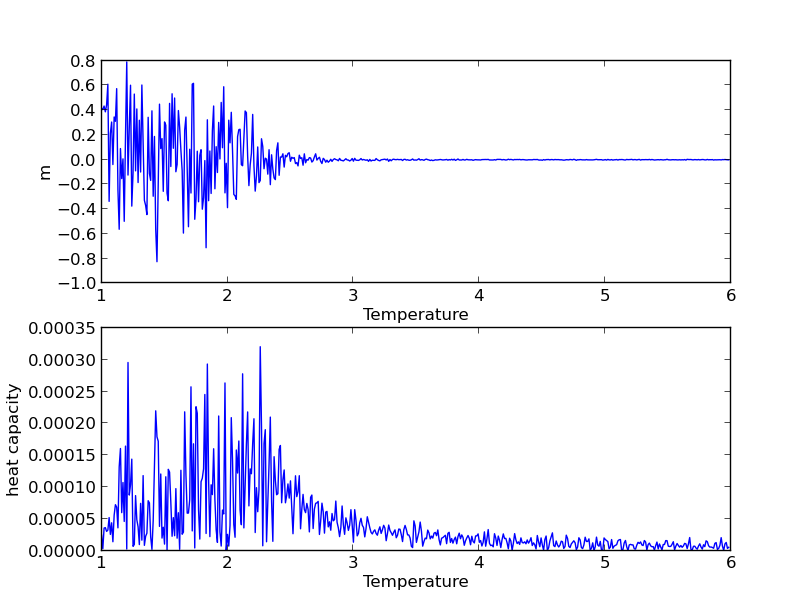
\includegraphics[width=0.8\linewidth,angle=0]{cp2100.png}
\caption{100x100 lattice m and c vs. T}
\label{figure6}
\end{center}
\end{figure}


We can see for larger lattice, since I didn't use enough number of steps, the pattern is not as obvious as that of 10x10, yet we can still see the shape of it.
To better evaluate the transition temperature, I applied FFT and got rid of the high frequency waves, as you can see in this plot: ~\ref{figure7} ~\ref{figure8} ~\ref{figure9}. 


\begin{figure}
\begin{center}
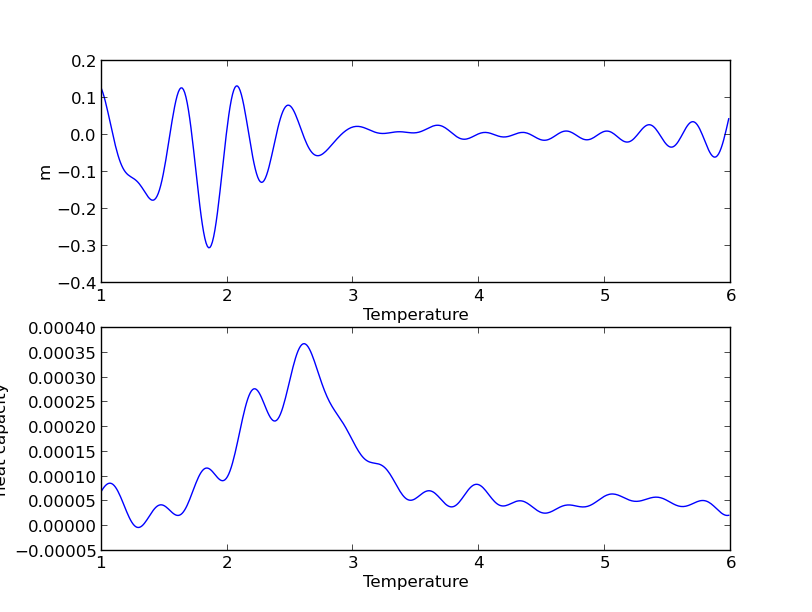
\includegraphics[width=0.8\linewidth,angle=0]{p2fft10.png}
\caption{10x10 fft lattice m and c vs. T}
\label{figure7}
\end{center}
\end{figure}

\begin{figure}
\begin{center}
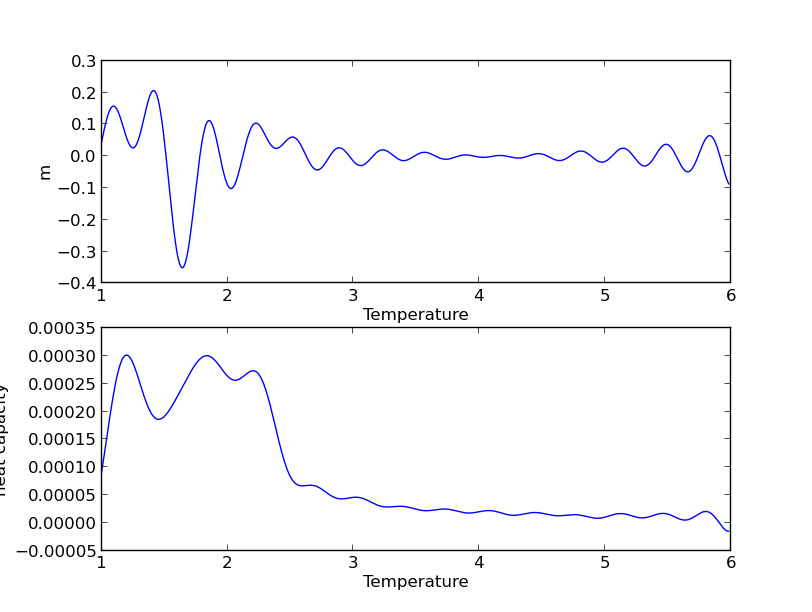
\includegraphics[width=0.8\linewidth,angle=0]{p2fft.png}
\caption{50x50 fft lattice m and c vs. T}
\label{figure8}
\end{center}
\end{figure}

\begin{figure}
\begin{center}
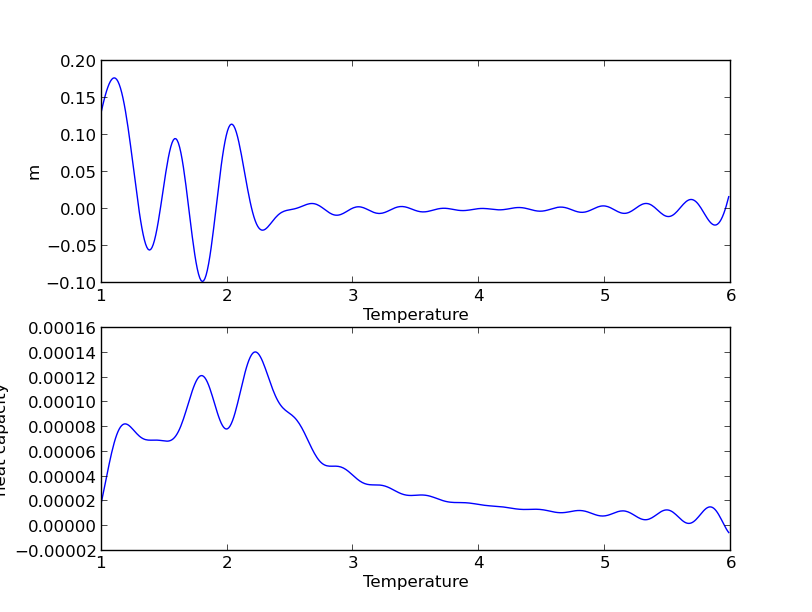
\includegraphics[width=0.8\linewidth,angle=0]{p2fft100.png}
\caption{100x100 fft lattice m and c vs. T}
\label{figure9}
\end{center}
\end{figure}

After fft, we can see for 10x10, 50x50, 100x100, the $T_c=2.62,2.22,2.23$ We can see later in the third problem, when the lattice is infinitely large, approximately the $T_c=2.27$, my result here is really close, considering the limit on the size and the random nature of the algorithm. I am going to use chi-square fit later in problem 3


\section{Problem 3}
\subsection{Description}

\begin{figure}
\begin{center}
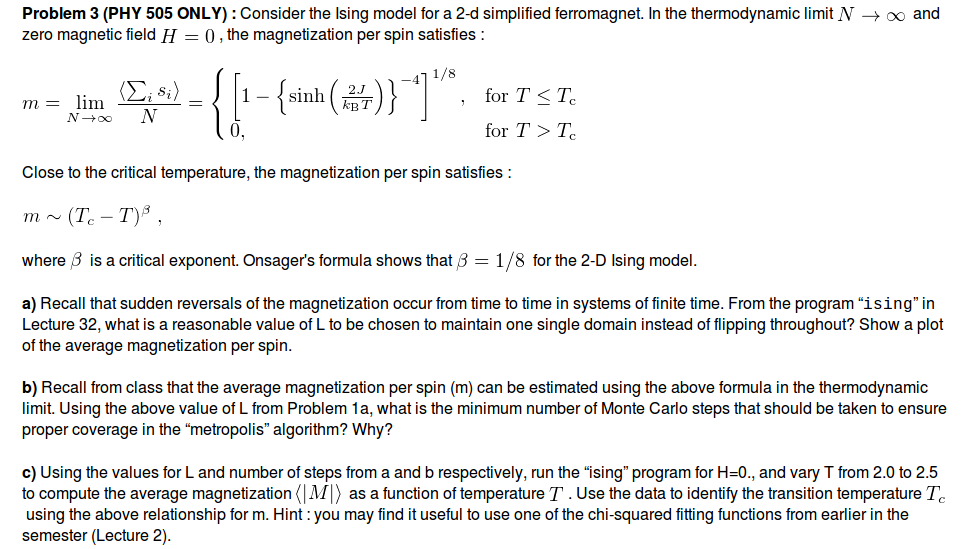
\includegraphics[width=0.8\linewidth,angle=0]{p3.png}
\caption{p3 description, sorry I am a little lazy}
\label{figure10}
\end{center}
\end{figure}


\subsection{Result}
\subsubsection{a}
To theoretically determine the proper number of L require probability theory and using Gaussian distribution. Yet that might be too troublesome here, after several trials I found L=30 should be a reasonable number. Here is the plot: ~\ref{figure11}

\begin{figure}
\begin{center}
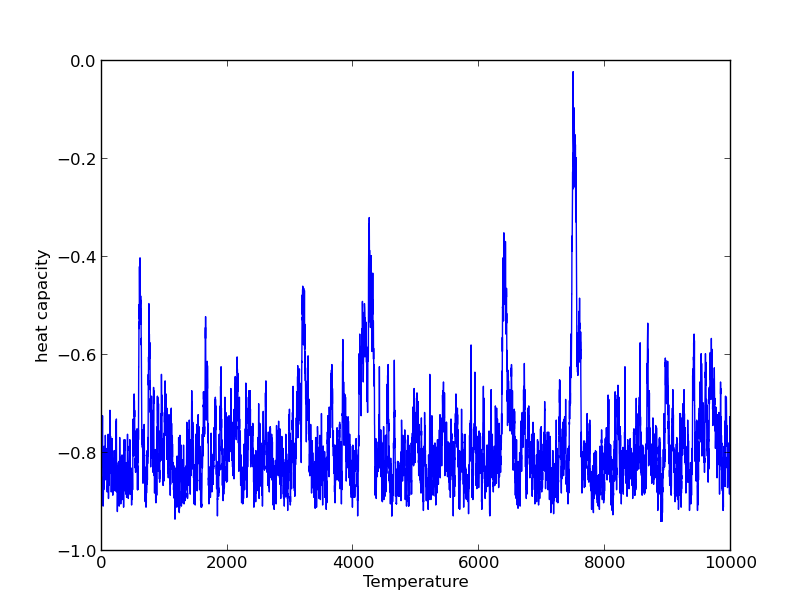
\includegraphics[width=0.8\linewidth,angle=0]{p3a.png}
\caption{30x30 average magnetization vs. steps}
\label{figure11}
\end{center}
\end{figure}

\subsubsection{b}
I firstly found all the Boltzmann factors are:0.026347980814448734\\
 37.95357249735125\\
 0.16232061118184818\\
  6.160647084304639\\1.0\\ 1.0\\6.160647084304639\\ 0.16232061118184818\\37.95357249735125\\ 0.026347980814448734\\
According the the Metropolis algorithm, firstly we have fifty fifty chance to have a spin=1 or 0($s_i$), for spin=0, the factor will always be 0 and this trial will not be used. For spin=1, after multiplying with Boltzmann factor, we can see six out of nine B-factors is larger than 1 and when times them, the trial will be effective. For other three, we can roughly think the chance the trial can be used is 0.11($\frac{1}{3}\times0.1623\times2+\frac{1}{3}\times0.026$). Thus, the chance one trial can be used is $0.5\times(\frac{2}{3}+0.11)=0.388$. A fair number of steps should satisfy that the expectation flipping number for individual spin greater than 1. Giving $N>L*L/0.388=2318$ I will say  2500 steps for simplicity.

\subsubsection{c}
Using the parameters above and I applied two chi-squared fits in two small ranges symmetric about a estimation of $T_c$, then find the intersect of these two lines. I found $T_c=2.272$, very close to the predicted value. Fig. ~\ref{figure12}  

\begin{figure}
\begin{center}
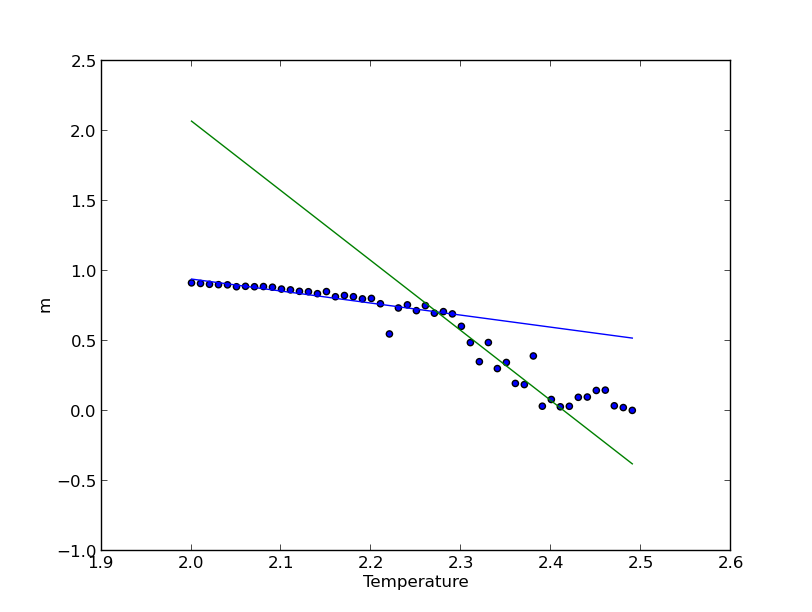
\includegraphics[width=0.8\linewidth,angle=0]{p3c.png}
\caption{30x30 average magnetization vs. temperature}
\label{figure12}
\end{center}
\end{figure}


\newpage
\section*{Acknowledgements}

I discussed this assignment with my classmates and used material from the
cited references, but this write-up is my own.

\begin{thebibliography}{9}


\bibitem{coursepage}
PHY 410-505 Webpage, \url{http://www.physics.buffalo.edu/phy410-505}.



\end{thebibliography}

\newpage
\appendix
\section{Appendix}

\subsection{python code}

The following python code was used to obtain the results in this report:

\lstinputlisting[language=c++]{ising.cpp}

\lstinputlisting[language=python]{isingp2.py}

\lstinputlisting[language=python]{plot.py}



\end{document}
